%264
\newpage
\subsection{条件判断の使い方}

今回もまず、プログラミングのツールHSP(Hot Soup Processor)を起動して、プログラムを実行するための準備を始めましょう。左上のRaspberry Piメニューの「プログラミング」項目にある、「HSP Script Editor」(HSPスクリプトエディタ)からエディタを起動してください。


\begin{figure}[H]
    \begin{center}
      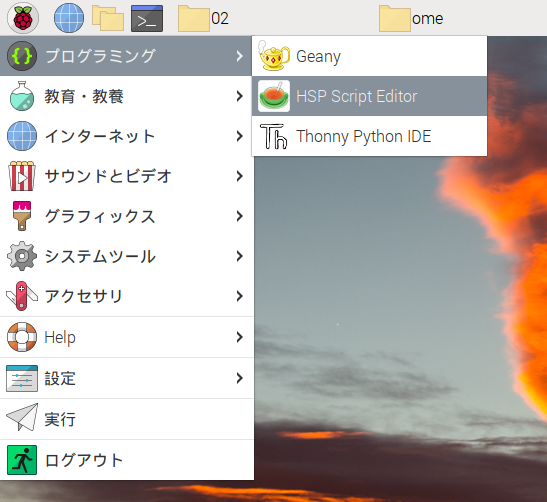
\includegraphics[keepaspectratio,width=7.31cm,height=6.562cm]{text04-img/s_hspmenu.png}
      \caption{プログラミング項目のメニュー}
    \end{center}
    \label{fig:prog_menu}
\end{figure}


いつも通りに、HSPスクリプトエディタを起動して作業を始めていきましょう。

\begin{figure}[H]
    \begin{center}
      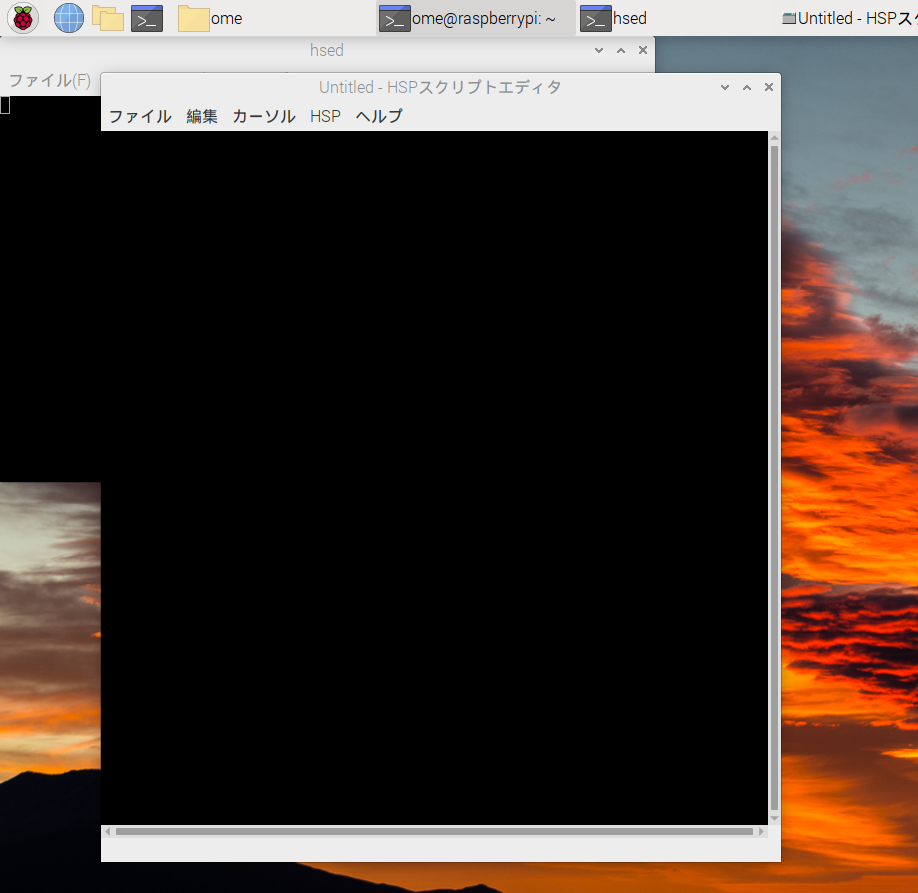
\includegraphics[keepaspectratio,width=7.31cm,height=6.562cm]{text04-img/s_hsed.png}
      \caption{HSPスクリプトエディタを起動したところ}
    \end{center}
    \label{fig:prog_menu}
\end{figure}



まずは、教材のプログラムを動かして試してみましょう。

ファイル→「開く」メニューから /home/ユーザー名/04 フォルダの中にある「swhandan.hsp」を読み込んでください。
作業は、すべて「/home/ユーザー名/04」フォルダで行ないます。

見つからない場合は、まわりの友達か、近くの先生に聞いてみてください。


\begin{figure}[H]
    \begin{center}
      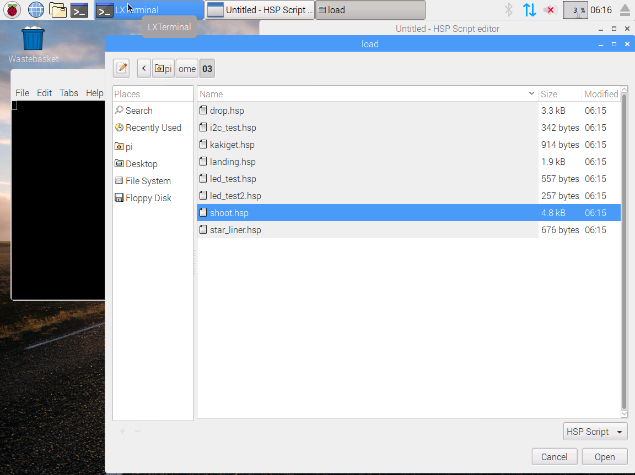
\includegraphics[keepaspectratio,width=7.338cm,height=5.493cm]{text04-img/text04-img002.png}
      \caption{フォルダから読み込む画面}
    \end{center}
    \label{fig:prog_menu}
\end{figure}


「swhandan.hsp」は、センサーボード上のスイッチを押すとメッセージが変わるかんたんなプログラムです。早速、[F5]キーを押して実行してみましょう。
%330


\begin{figure}[H]
    \begin{center}
      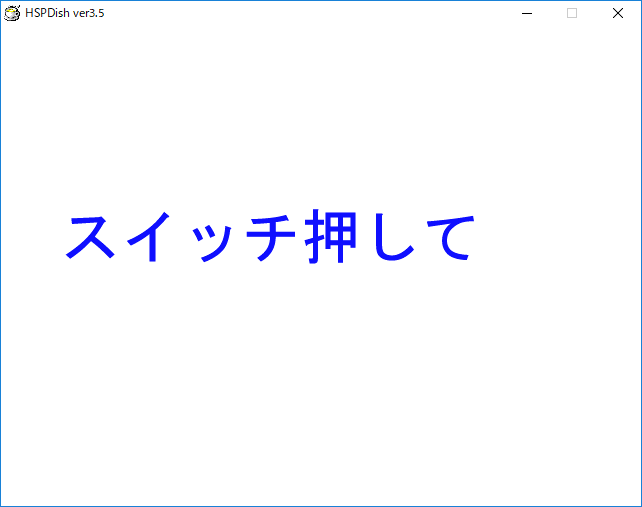
\includegraphics[keepaspectratio,width=7.673cm,height=6.05cm]{text04-img/text04-img003.png}
      \caption{swhandan.hspの実行画面}
    \end{center}
    \label{fig:prog_menu}
\end{figure}


%347